\textit{Примечание:} везде, если не оговорено иное, имеются в виду правые и левые берега рек \textbf{орографически}.
\subsection{18 августа. Старт}
\textit{Метеоусловия: утром, днём, вечером ясно, тепло.}

\begin{figure}[h!]
	\centering
	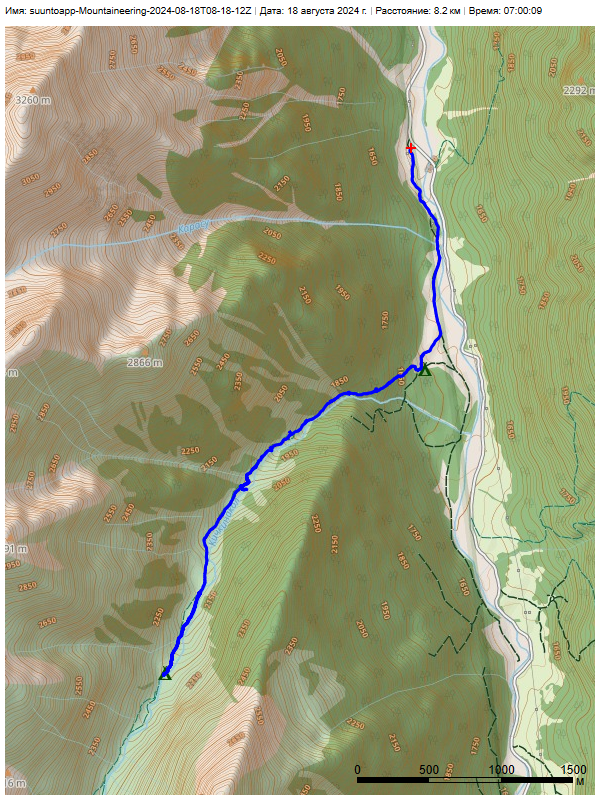
\includegraphics[angle=0, width=0.7\linewidth]{../pics/mini_maps/18}
	\label{fig:mini_18}
\end{figure}


Приезжаем в г. Минеральные Воды в 03:40. Встречаемся на вокзале с участником, прибывшим на день раньше и загружаемся в машину Бориса Саракуева. В 04:00 отправляемся на место старта (мост через р. Учкулан, N 43.38668\degree~E 41.98961\degree), куда прибываем в 09:45 (По дороге на 40 минут остановились в ауле Учкулан, чтобы позавтракать). Распределяем заброски, отдаём их водителю и выдвигаемся на маршрут в 11:18. Первые 1.5 км до коша проходим по д.р. Учкулан, затем тропа проходит через калитку и поворачивает направо, на подъём в висячую долину р. Кичкинакол Джалпаккольский.

\begin{figure}[h!]
	\centering
	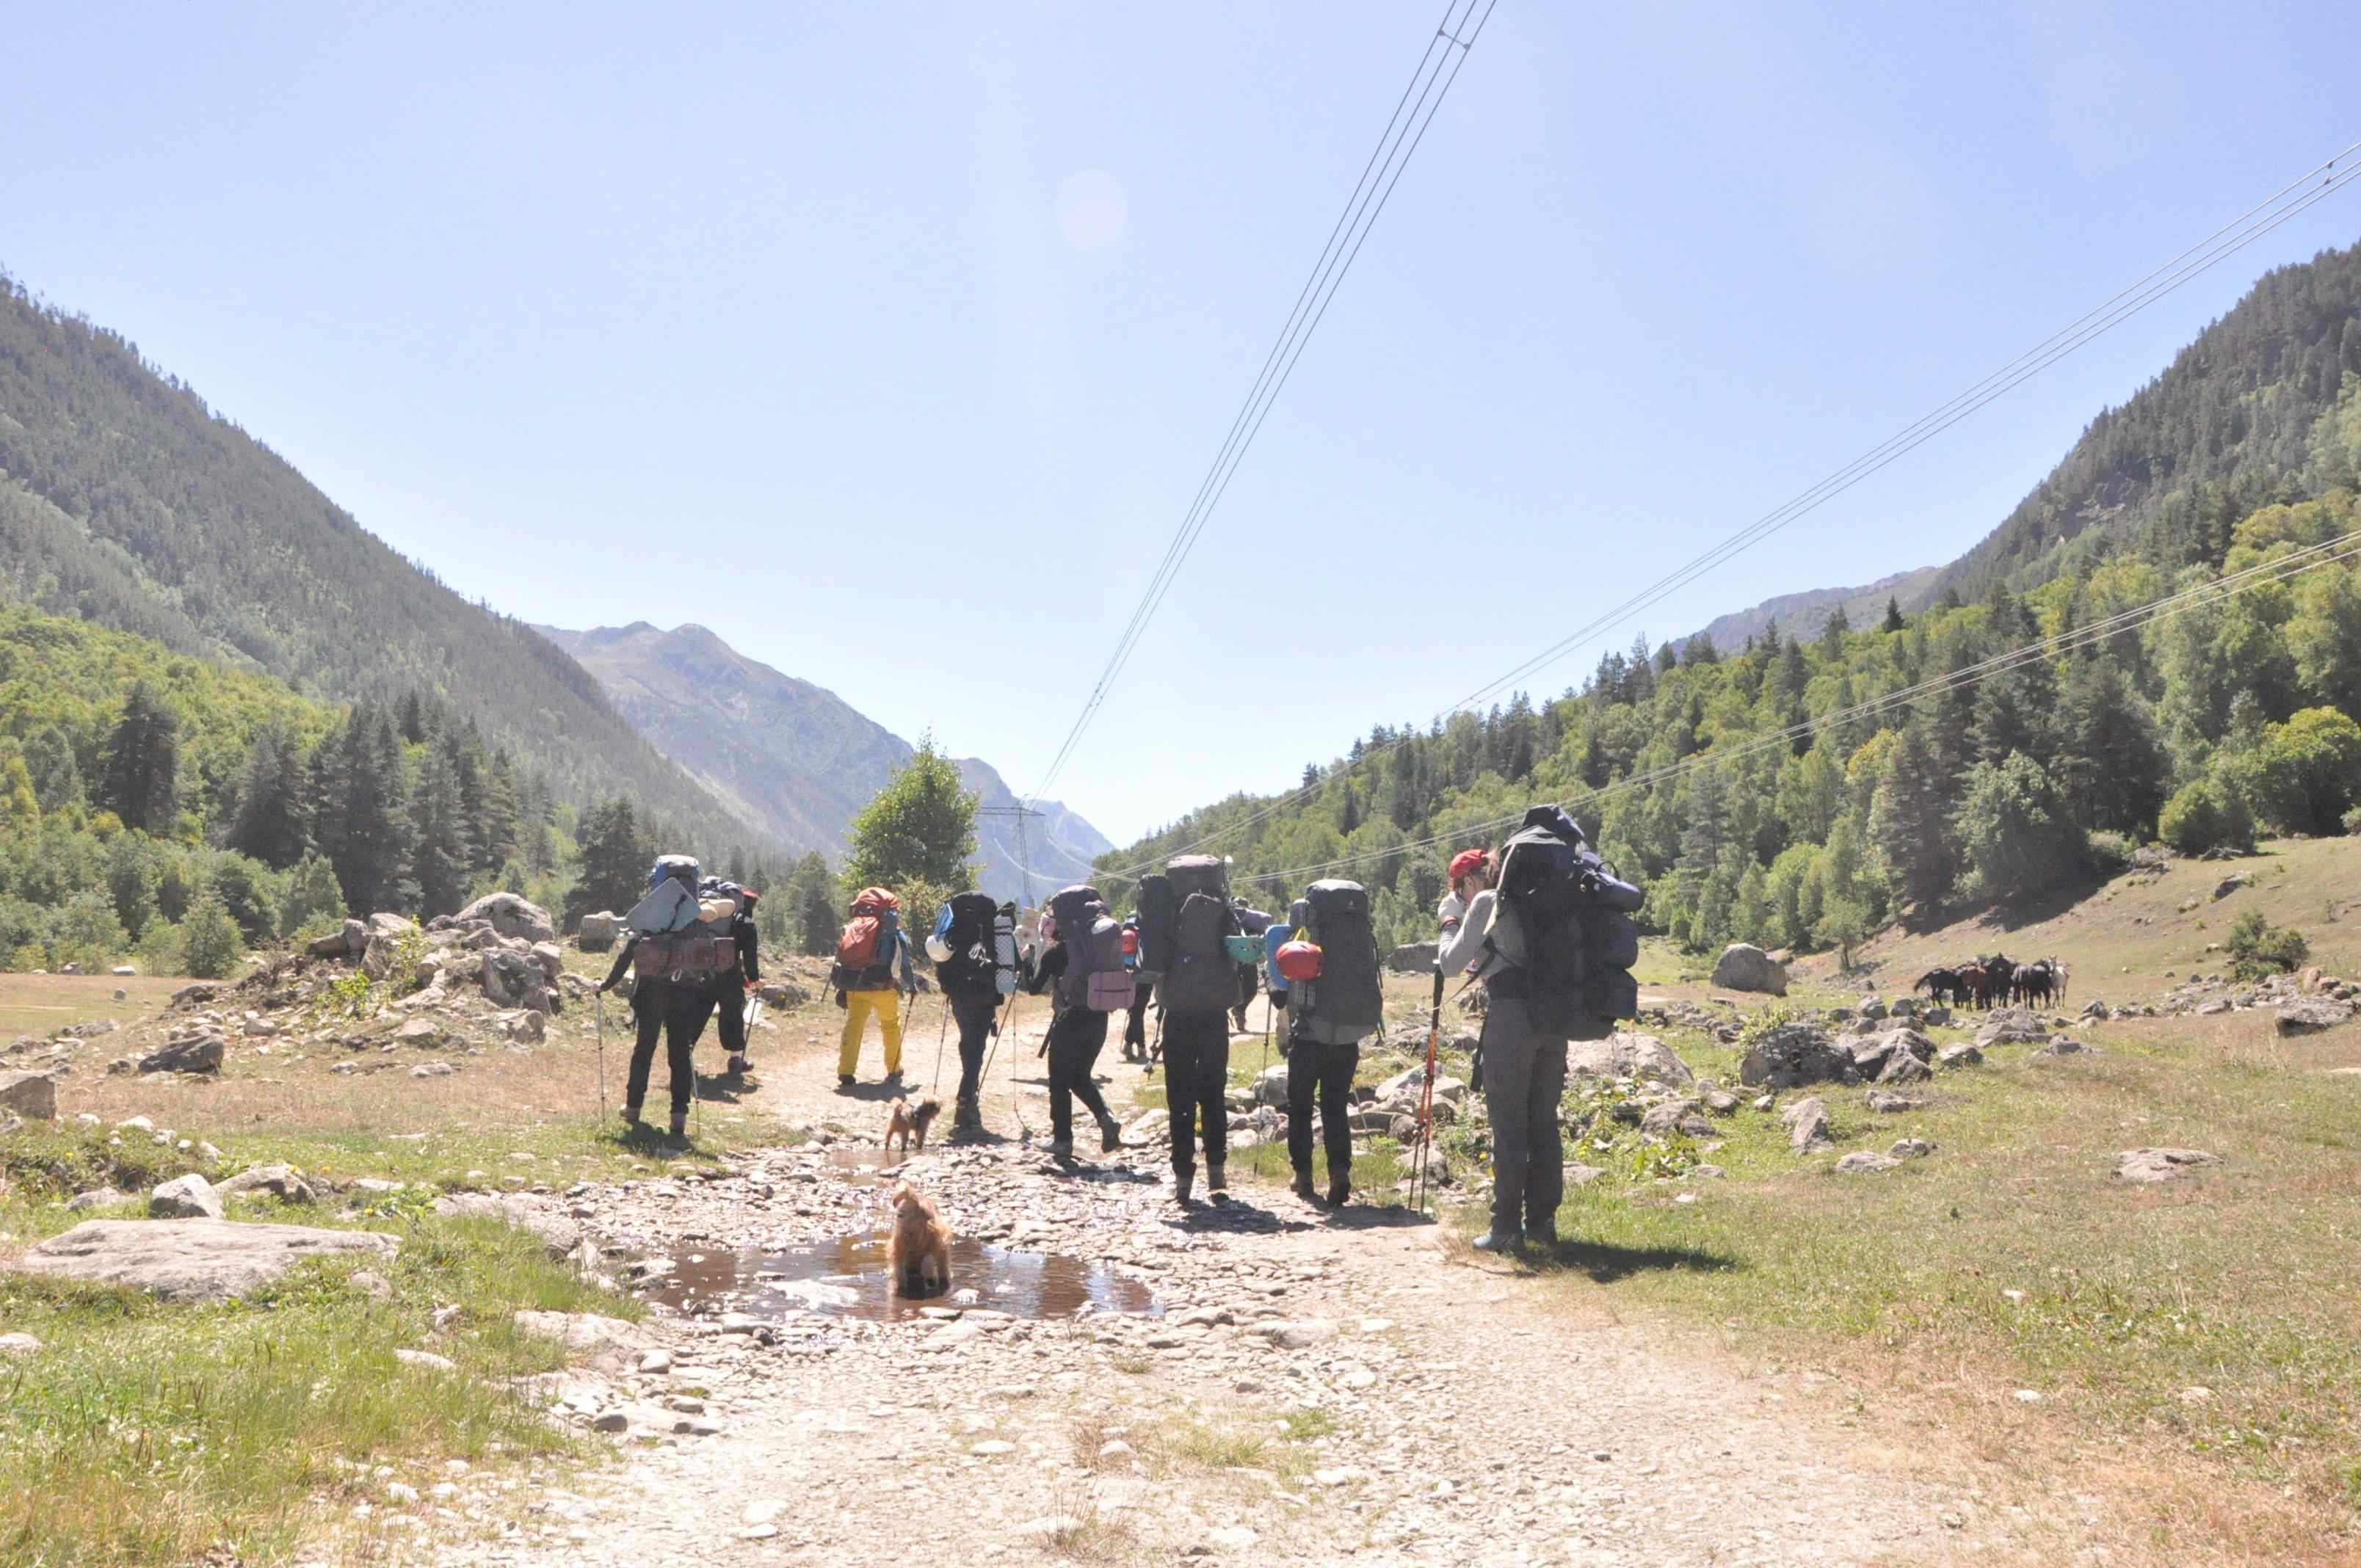
\includegraphics[width=0.7\linewidth]{../pics/DSC_0412}
	\caption{группа на старте маршрута в д.р. Учкулан}
	\label{fig:uchkulan}
\end{figure}


\begin{figure}[h!]
	\centering
	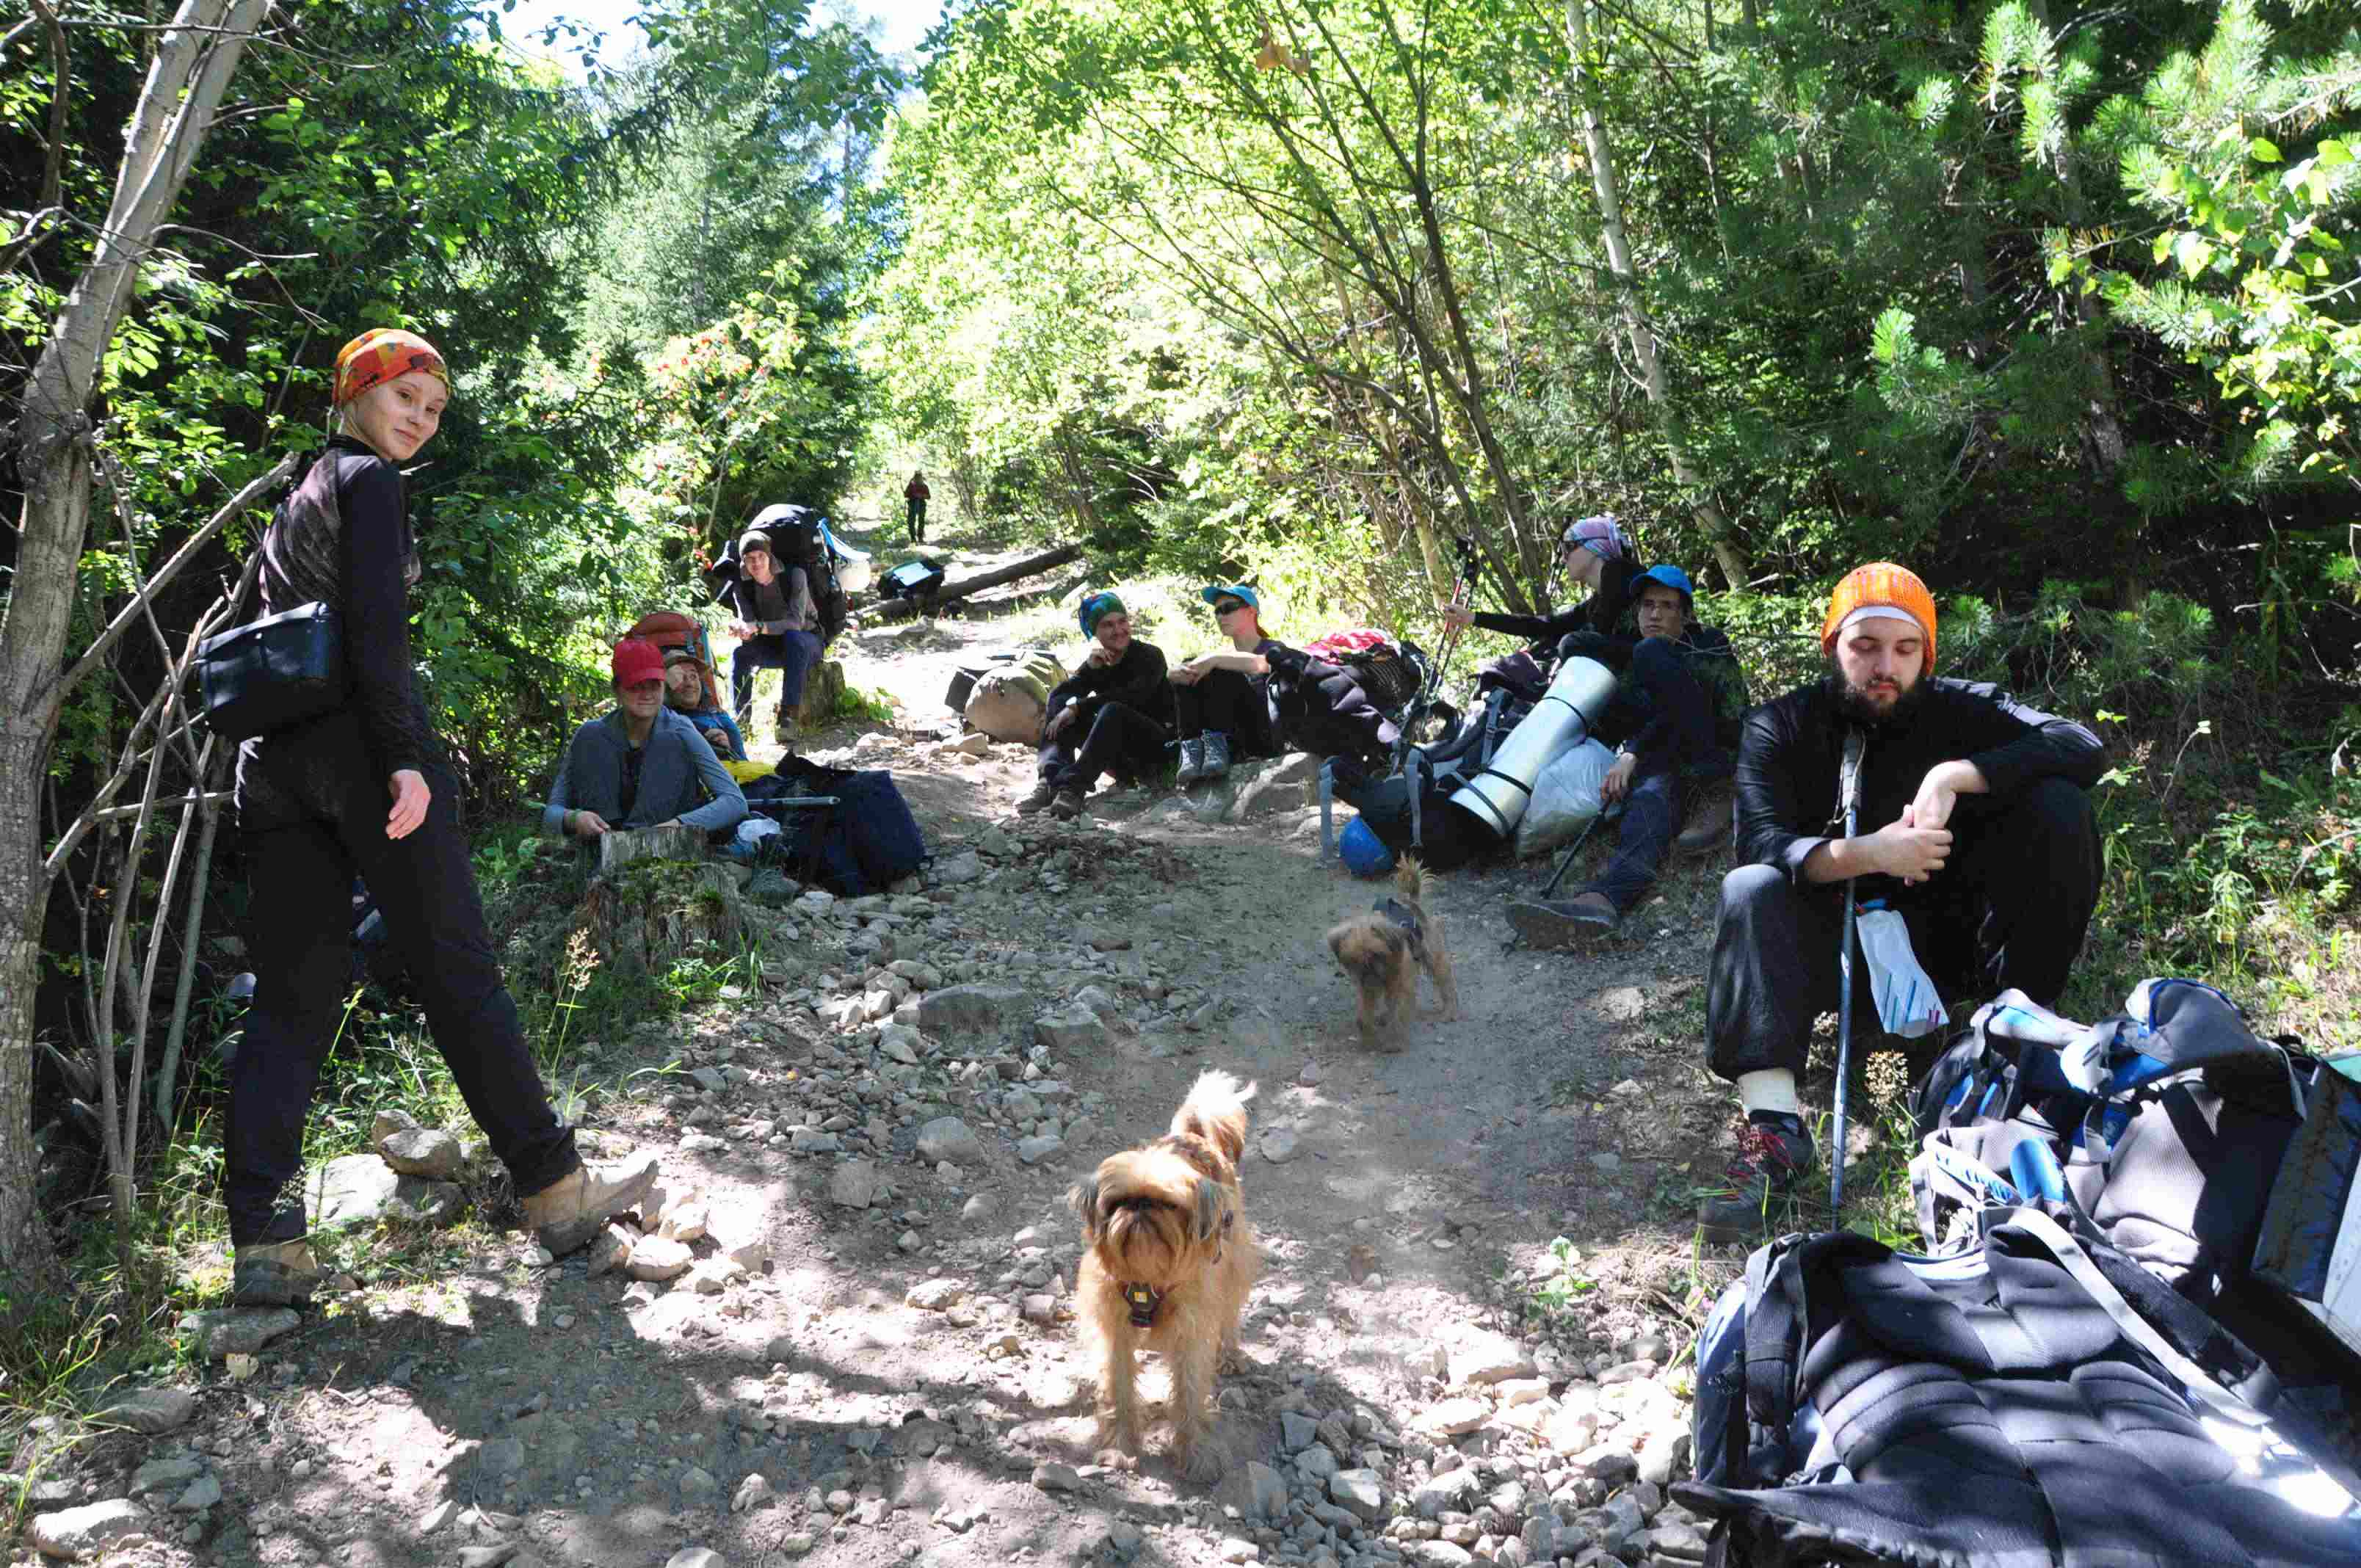
\includegraphics[width=0.7\linewidth]{../pics/DSC_0436}
	\caption{Подъём по тропе в д.р. Кичкинакол Уллукёльский}
	\label{fig:DSC_0436}
\end{figure}

Подъём в висячую долину идёт по хорошей тропе со средний уклоном порядка 20\degree (рис.~\ref{fig:DSC_0436}). Идём не спеша, в режиме 20/5, разгружаем отстающих участников. В 14:30 заканчиваем подъём в долину и устраиваем обед.

\begin{figure}[h!]
	\centering
	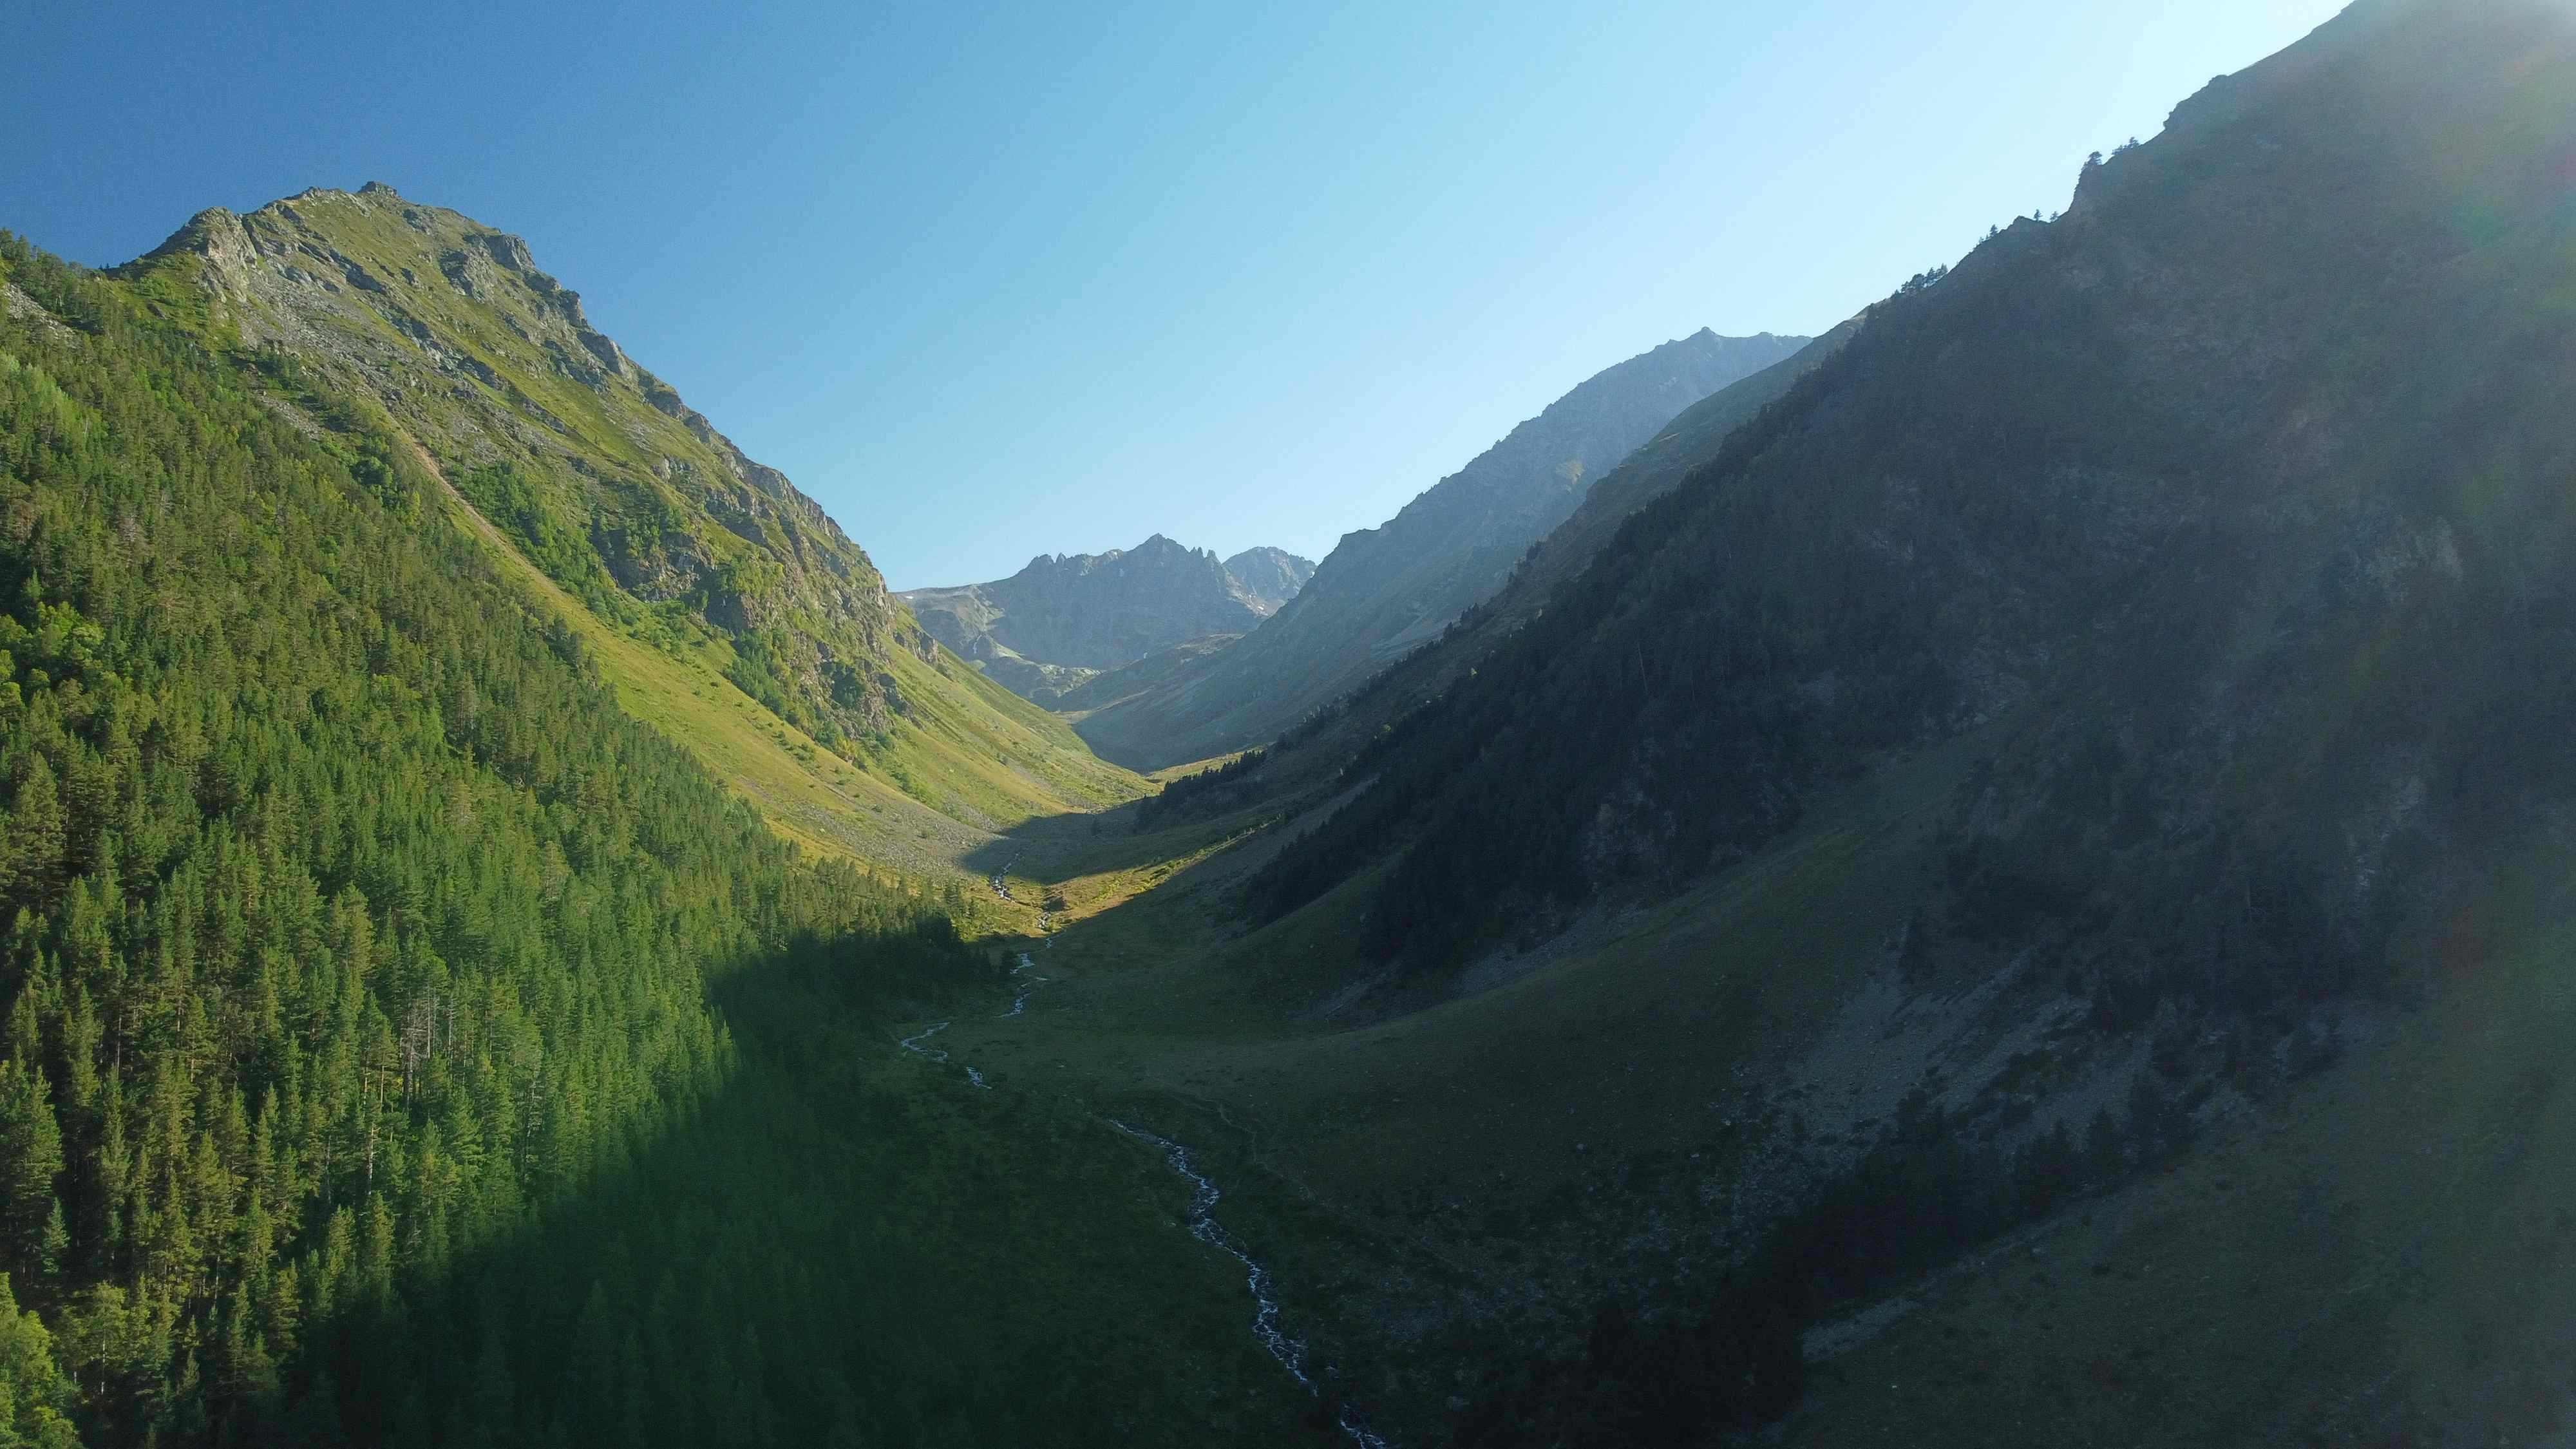
\includegraphics[width=0.7\linewidth]{../pics/DJI_0805}
	\caption{д.р. Кичкинакол Джалпаккольский}
	\label{fig:kichkinakol}
\end{figure}

Заканчиваем обед в 16:40 и проходим 2 км к оборудованной стоянке возле коша, где оказываемся в 17:25. Рядом местные жители собирают малину. Подумав немного и устроив разведку, поднимаемся ещё немного выше и в 18:18 встаём на место ночёвки на оборудованной стоянке возле дерева на небольшом разливе реки. Координаты м.н. N 43.35392\degree~E 41.96858\degree.
\begin{figure}[h!]
	\centering
	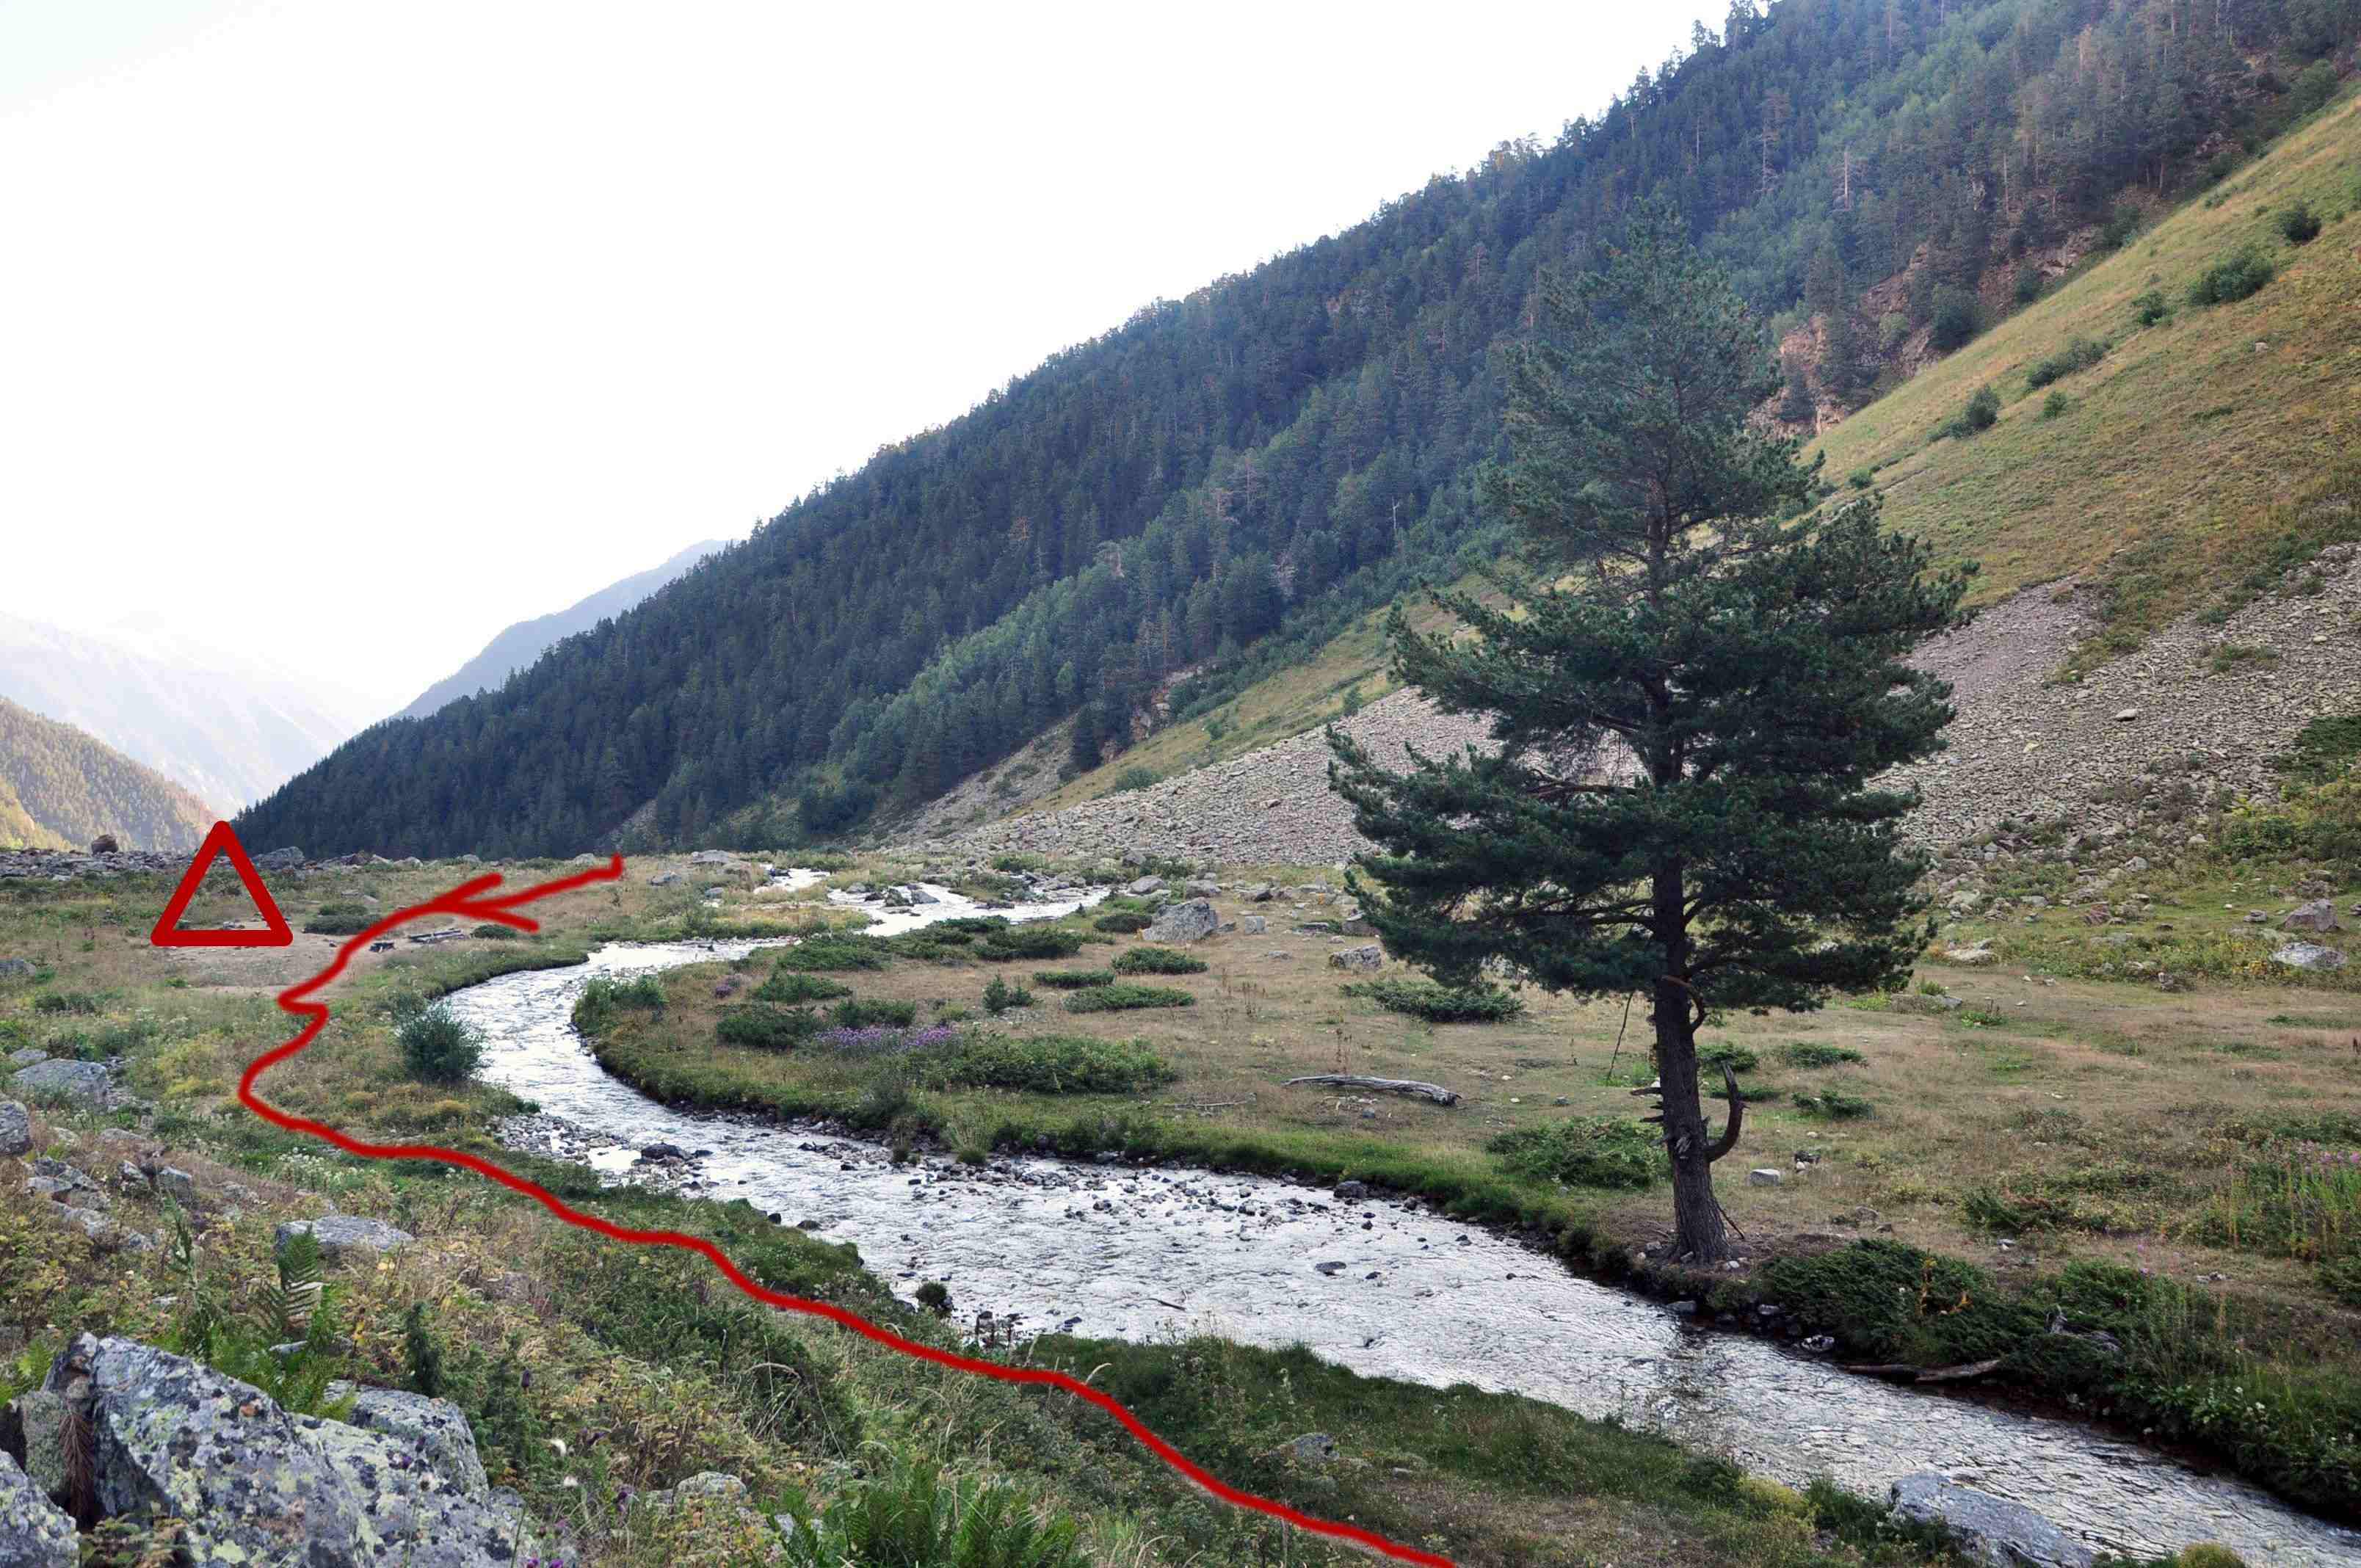
\includegraphics[width=0.7\linewidth]{../pics/camp_18}
	\caption{Место ночёвки 18-19.08}
	\label{fig:camp_18}
\end{figure}


\newpage